\documentclass[12pt]{amsart}

\addtolength{\hoffset}{-2.25cm}
\addtolength{\textwidth}{4.5cm}
\addtolength{\voffset}{-2.5cm}
\addtolength{\textheight}{5cm}
\setlength{\parskip}{0pt}
\setlength{\parindent}{15pt}
\usepackage{listings}
\usepackage{amsthm}
\usepackage{amsmath}
\usepackage[spanish]{babel}
\usepackage[sort&compress, numbers]{natbib}
\usepackage{amssymb}
\usepackage[utf8]{inputenc}
\usepackage[colorlinks = true, linkcolor = black, citecolor = black, final]{hyperref}


\usepackage{graphicx}
\usepackage{multicol}
\usepackage{ marvosym }
\newcommand{\ds}{\displaystyle}


\pagestyle{myheadings}

\setlength{\parindent}{0in}
\begin{document}

\pagestyle{empty}



\thispagestyle{empty}

{\scshape Simulación} \hfill {\scshape \Large Tarea 1: Movimiento Browniano} \hfill  {\scshape 24/Feb/2021}
\author{C. María Montemayor Palos}
\maketitle

\hrule
\hrule
\bigskip


\section{Objetivo}
El objetivo de esta práctica es examinar sistemáticamente los efectos de la dimensión en el tiempo de regreso al origen del movimiento Browniano para dimensiones uno a cinco en incrementos lineales de uno, variando el número de pasos de la caminata como potencias de dos con exponente de cuatro a nueve en incrementos lineales de uno, realizando treinta repeticiones del experimento para cada combinación.

\section{Metodología}
Se utilizó el programa R versión 4.0.4 \cite{R} para Windows para llevar a cabo el movimiento Browniano. Se generó un código para evaluar el tiempo del regreso al origen de una partícula que se mueve al azar, tomando como código base la rutina de caminata \cite{Dra.Elisa} de la partícula.

Se variaron los pasos de la caminata con potencias de dos con exponentes de cuatro a nueve programando treinta repeticiones para cada experimento en dimensiones de uno a cinco. Se tomó como apoyo el repositorio de CrisAE \cite{CrisAE}.

\section{Código}
Se muestra una parte del código en la cual se determinan las dimensiones con pasos de dos elevado a los exponentes de cuatro a nueve respectivamente.
\begin{lstlisting}
for (dim in 1:5){ #en dimensiones de 1 a 5
  for(expo in 4:9){ #exponencial de 4 a 9
    caminata <- 2**expo #en pasos de 2 elevado a los exponentes
    origenes<-numeric()
    for(replica in 1:30){ #en repeticiones de 1 a 30
      origenes<- c(origenes, movpar(dim, caminata))
      movpar<-function(dim, caminata){
        par <- rep(0,dim)
        regreso<-TRUE
        for(t in 1:caminata){
          cambiar <- sample(1:dim,1)
          if(runif(1)<0.5){
            par[cambiar] <- par[cambiar] + 1
          }else{
            par[cambiar] <- par[cambiar]-1
          }
          if(all(par==0)){
            return(t)


\end{lstlisting}

\section{Resultados y discusión}
Para observar su efecto en el tiempo de regreso al punto de origen de la partícula, se aumentaron de manera lineal los pasos de 2 con exponentes de 4 a 9 como se aprecia en los siguientes cuadros. 
{
\bigskip
\medskip
\begin{table}[ht]
    \caption{Caminata de 16 pasos: $dimensión$ de uno a cinco respectivamente en la que se mueve la partícula, después se proporcionan los valores de mínimo, máximo, promedio ($\mu$) y el porcentaje (\%) de partículas que nunca regresaron.}
    \label{datos}
    \centering
    \begin{tabular}{|r|rrr|r|}
       \hline
        $dimensión$&$mín$&$máx$&$\mu$&\% \\
        \hline
        1 & 2 & 10 & 2 & 1.3 \\
        2 & 2 & 12 & 4 & 43.33 \\
        3 & 2 & 2 & 2 & 86.66 \\
        4 & 2 & 4 & 2.5 & 86.66 \\
        5 & 2 & 10 & 4 & 83.33\\
        \hline
    \end{tabular}
\end{table}
\bigskip

\begin{table}[ht]
    \caption{Caminata de 32 pasos}
    \label{datos}
    \centering
    \begin{tabular}{|r|rrr|r|}
       \hline
        $dimensión$&$mín$&$máx$&$\mu$&\% \\
        \hline
        1 & 2 & 20 & 2 & 2 \\
        2 & 2 & 18 & 4 & 43.33 \\
        3 & 2 & 2 & 3.5 & 73.33 \\
        4 & 2 & 4 & 2.6 & 90 \\
        5 & 2 & 4 & 2.6 & 90\\
        \hline
    \end{tabular}
\end{table}
\bigskip

\begin{table}[ht]
    \caption{Caminata de 64 pasos}
    \label{datos}
    \centering
    \begin{tabular}{|r|rrr|r|}
       \hline
        $dimensión$&$mín$&$máx$&$\mu$&\% \\
        \hline
        1 & 2 & 8 & 2.7 & 3 \\
        2 & 2 & 12 & 9.33 & 40 \\
        3 & 2 & 36 & 3.5 & 63.33 \\
        4 & 2 & 2 & 2 & 93.33 \\
        5 & 2 & 2 & 2 & 90\\
        \hline
    \end{tabular}
\end{table}
\bigskip

\begin{table}[ht]
    \caption{Caminata de 128 pasos}
    \label{datos}
    \centering
    \begin{tabular}{|r|rrr|r|}
       \hline
        $dimensión$&$mín$&$máx$&$\mu$&\% \\
        \hline
        1 & 2 & 36 & 5.5 & 3 \\
        2 & 2 & 12 & 9.33 & 30 \\
        3 & 2 & 116 & 16.67 & 53.33 \\
        4 & 2 & 8 & 3.6 & 83.33 \\
        5 & 2 & 2 & 2 & 90\\
        \hline
    \end{tabular}
\end{table}
\bigskip

\begin{table}[ht]
    \caption{Caminata de 256 pasos}
    \label{datos}
    \centering
    \begin{tabular}{|r|rrr|r|}
       \hline
        $dimensión$&$mín$&$máx$&$\mu$&\% \\
        \hline
        1 & 2 & 36 & 11.6 & 100 \\
        2 & 2 & 130 & 9.3 & 80 \\
        3 & 2 & 30 & 6.5 & 63.33 \\
        4 & 2 & 16 & 4.8 & 83.33 \\
        5 & 2 & 2 & 2.6 & 90\\
        \hline
    \end{tabular}
\end{table}
\bigskip

\begin{table}[ht]
    \caption{Caminata de 512 pasos}
    \label{datos}
    \centering
    \begin{tabular}{|r|rrr|r|}
       \hline
        $dimensión$&$mín$&$máx$&$\mu$&\% \\
        \hline
        1 & 2 & 58 & 7.03 & 3.33 \\
        2 & 2 & 154 & 21.3 & 33.33 \\
        3 & 2 & 124 & 19.6 & 66.66 \\
        4 & 2 & 36 & 6.7 & 73.33 \\
        5 & 2 & 14 & 6.6 & 90\\
        \hline
    \end{tabular}
\end{table}
}
\\
\\
\\
\bigskip
\bigskip
\bigskip
\bigskip
\bigskip
Se generó un diagrama de caja-bigote (ver figura 1) para visualizar de manera gráfica la distancia máxima de caminata de la partícula en las cinco dimensiones.
\bigskip
\begin{figure}[h!]
    \centering
    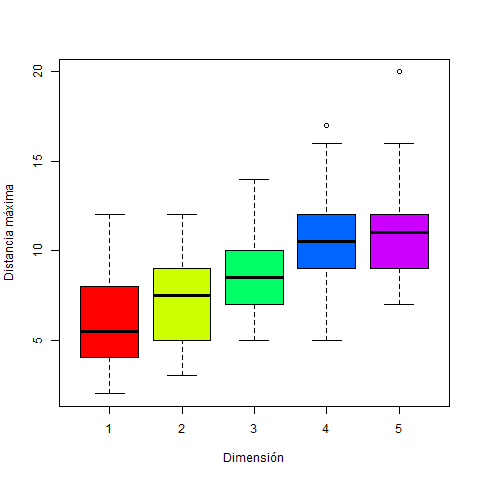
\includegraphics[width=0.5\textwidth]{p1mr.png}
    \caption{\label{fig1}Diagrama caja-bigote}
    \label{fig:figura1}
\end{figure}

Se puede concluir que la partícula tarda más en regresar al punto de origen o regresa un menor número de veces cuando se encuentra en la dimensión 5, por lo tanto entre menor sea la cantidad de dimensiones, mayor será el tiempo de regreso de la partícula al punto de origen.
\bigskip
\bigskip
\bigskip
\bigskip
\bigskip
\bigskip
\bibliography{Dra.Elisa}
\bibliographystyle{plainnat}


\bigskip

\end{document}


